\documentclass[parskip=full]{scrartcl}

\pdfoutput=1

\usepackage{breakcites}
\usepackage[square,numbers]{natbib}
\usepackage{float}
\usepackage{graphicx}
\usepackage{geometry}
\geometry{%
	a4paper,
	left=18mm,
	right=18mm,
	top=18mm,
}
\usepackage{amsmath}
\usepackage{enumitem}
\usepackage[ruled,vlined]{algorithm2e}
\usepackage{booktabs}
\usepackage{pgfplotstable}
\pgfplotsset{compat=1.14}
\usepackage{longtable}
\usepackage{tabu}
\usepackage{hyperref}
\date{}

\definecolor{hypecol}{HTML}{0875b7}
\hypersetup{%
    colorlinks,
    linkcolor={hypecol},
    citecolor={hypecol},
    urlcolor={hypecol}
}

\title{%
    Heuristic Data Augmentation Improves the Efficiency of Active Learning
    Methods
}

\author{%
	Joao Fonseca\(^{1*}\), Fernando Bacao\(^{1}\)
	\\
	\small{\(^{1}\)NOVA Information Management School, Universidade Nova de Lisboa}
	\\
	\small{*Corresponding Author}
	\\
	\\
	\small{Postal Address: NOVA Information Management School, Campus de
    Campolide, 1070--312 Lisboa, Portugal}
	\\
	\small{Telephone: +351 21 382 8610}
}

\begin{document}

\maketitle

\begin{abstract}
    Abstract goes here.
\end{abstract}

\section{Introduction}

Introduction goes here.

\section{Active Learning Methods}

Review on Data Augmentation Methods go here.

\section{Data Augmentation Methods}

Review on Data Augmentation Methods go here.

% discuss G-SMOTE

\section{Proposed Method}~\label{sec:proposed_method}

\section{Methodology}~\label{sec:methodology}

This section describes the different elements included in the experimental
procedure. The datasets used were acquired in open data repositories and its
sources and preprocessing steps are defined in Subsection~\ref{sec:datasets}.
The choice of classifiers used in the experiment are defined in
Subsection~\ref{sec:machine_learning_algorithms}. The metrics chosen to
measure AL performance and overall classification performance are defined in
Subsection~\ref{sec:evaluation_metrics}. The experimental procedure is
described in Subsection~\ref{sec:experimental_procedure}. The implementation
of the experiment and resources used to do so are described in
Subsection~\ref{sec:software_implementation}.

The methodology developed serves 2 purposes: (1) Compare classification
performance once all the AL procedures are completed (\textit{i.e.,} optimal
performance of a classifier trained via iterative data selection) and (2)
Compare the amount of data required to reach specific performance thresholds
(\textit{i.e.,} number of AL iterations required to reach similar the optimal
classification performance).

\subsection{Datasets}~\label{sec:datasets}

The datasets used to test the proposed method are publicly available in open
data repositories. Specifically, they were retrieved from
\href{https://www.openml.org/}{OpenML} and the
\href{https://archive.ics.uci.edu/}{UCI Machine Learning Repository}. The
datasets were chosen considering different domains of application, imbalance
ratios, dimensionality and number of target classes, all of them focused on
classification tasks. The goal is to demonstrate the performance of the
different AL frameworks in various scenarios and domains. The data
preprocessing approach was similar across all datasets.
Table~\ref{tab:datasets_description} describes the key properties of the 10
preprocessed datasets where the experimental procedure was applied. 

\begin{table}[H]
    \centering
    \addtolength{\leftskip} {-2cm}
    \addtolength{\rightskip}{-2cm}
    \pgfplotstabletypeset[
        col sep=comma,
        string type,
        every head row/.style={%
            before row=\toprule,
            after row=\midrule
        },
        every last row/.style={after row=\bottomrule},
    ]{../analysis/datasets_description.csv}
    \caption{\label{tab:datasets_description}
        Description of the datasets collected after data preprocessing. The
        sampling strategy is similar across datasets. Legend: (IR) Imbalance
        Ratio
    }
\end{table}

The data preprocessing pipeline is depicted as a flowchart in
Figure~\ref{fig:data_preprocessing}. The missing values are removed from each
dataset by removing the corresponding observations. This ensures that the
input data in the experiment is kept as close to its original form as
possible. The non-metric features (\textit{i.e.,} binary, categorical and
ordinal variables) were removed since the application of G-SMOTE is limited to
continuous and discrete features. The datasets containing over 2000
observations were downsampled in order to maintain the datasets to a
manageable size. The data sampling procedure preserves the relative class
frequency of the dataset, in order to maintain the Imbalance Ratio (IR)
originally found in each dataset (where $IR =
\frac{count(C_{maj})}{count(C_{\min})}$). The remaining features of each
dataset are scaled to the range of $[-1, 1]$ to ensure a common range across
features.

\begin{figure}[H]
	\centering
	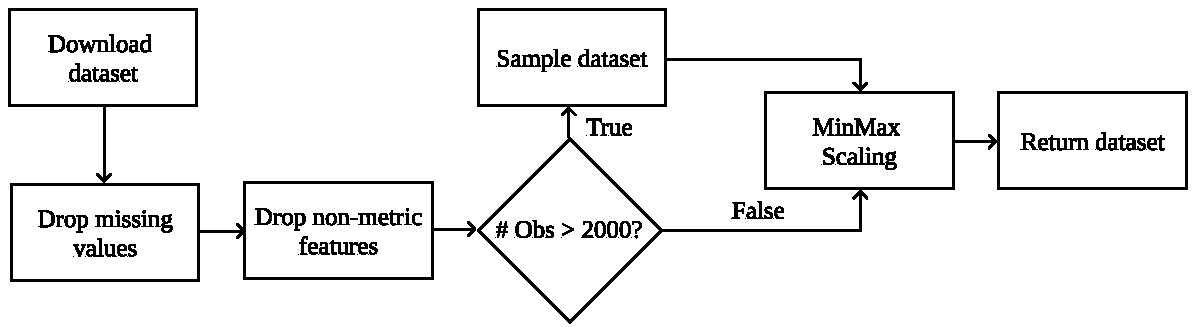
\includegraphics[width=1\linewidth]{../analysis/data_preprocessing}
    \caption{%
        Data preprocessing pipeline.
    }~\label{fig:data_preprocessing}
\end{figure}

The preprocessed datasets were stored into a SQLite database file and is
available along with the experiment's source code in the GitHub repository of
the project (see Subsection~\ref{sec:software_implementation}).

\subsection{Machine Learning Algorithms}~\label{sec:machine_learning_algorithms}

We used a total of 4 classification algorithms and a heuristic data
augmentation mechanism. The choice of classifiers was based on the popularity
and family of the classifiers (tree-based, nearest neighbors-based,
ensemble-based and linear models). Our proposed method was tested using a
Decision Tree (DT)~\cite{Wu1975}, a K-nearest neighbors classifier
(KNN)~\cite{Cover1967}, a Random Forest Classifier (RF)~\cite{Ho1995} and a
Logistic Regression (LR)~\cite{Nelder1972}. Since the target variables are
multi-class, the LR classifier was implemented using the one-versus-all
approach. The predicted class is assigned to the label with the highest
likelihood.

The oversampler G-SMOTE was used as a data augmentation method. The typical
sampling strategy of oversampling methods is to generate artificial
observations on non-majority classes such that the number of majority class
observations matches those of each non-majority class. We modified this
sampling strategy to generate observations for all classes, as a percentage of
the number of observations in the majority class. In addition, the original
G-SMOTE algorithm was modified to accept data selection probabilities based on
classification uncertainty. These modifications are discussed in
Section~\ref{sec:proposed_method}.

Every AL procedure was tested with different selection criteria: Random
Selection, Entropy and Breaking Ties. The baseline used is the standard AL
procedure. As a benchmark, we add the AL procedure using G-SMOTE as a normal
oversampling method, as proposed in~\cite{Fonseca2021}. Our proposed method
was implemented using G-SMOTE as a data augmentation method to generate
artificial observations for all classes, while still balancing the class
distribution, as described in Section~\ref{sec:proposed_method}. 

\subsection{Evaluation Metrics}~\label{sec:evaluation_metrics}

Considering the imbalanced nature of the datasets used in the experiment,
commonly used performance metrics such as Overall Accuracy (OA), although
being intuitive to interpret, are insufficient quantify a model's
classification performance~\cite{Jeni2013}. The Cohen's Kappa performance
metric, similar to OA, is also biased towards high frequency classes since its
definition is closely related to the OA metric, making its behavior consistent
with OA~\cite{Fatourechi2008}. However, these metrics remain popular choices
for the evaluation of classification performance. Other performance metrics
like $Precision = \frac{TP}{TP+TN}$, $Recall = \frac{TP}{TP+FN}$ or
$Specificity = \frac{TN}{TN + FP}$ are calculated as a function of True/False
Positives (TP and FP) and True/False Negatives (TN and FN) and can be used at
a per-class basis instead. In a multiple dataset with varying amount of target
classes and meanings, comparing the performance of different models using
these metrics becomes impractical.

Based on the recommendations found in~\cite{Jeni2013, Kubat1997}, we used 2
metrics found to be less sensitive to the class imbalance bias, along with OA
as a reference for easier interpretability:

\begin{itemize}
    \item The Geometric-mean scorer (G-mean) consists of the geometric mean of
        Specificity and Recall~\cite{Kubat1997}. Both metrics are calculated
        in a multiclass context considering a one-versus-all approach. For
        multiclass problems, the G-mean scorer is calculated as its average
        per class values: 
        
        \begin{equation*}
            \textit{G-mean} = \sqrt{\overline{Sensitivity} \times
            \overline{Specificity}}
        \end{equation*}

    \item The F-score metric consists of the harmonic mean of Precision and
        Recall. The two metrics are also calculated considering a
        one-versus-all approach. The F-score for the multi-class case
        can be calculated using its average per class values~\cite{Jeni2013}:

        \begin{equation*}
            \textit{F-score}=2\times\frac{\overline{Precision} \times
            \overline{Recall}}{\overline{Precision} + \overline{Recall}}
        \end{equation*}

    \item The OA consists of the number of TP divided by the total amount of
        observations. Considering $c$ as the label for the different classes
        present in a target class, OA is given by the following formula:

        \begin{equation*}
            \textit{OA} = \frac{\sum\limits_{c}{\text{TP}_{c}}}{%
		    	      \sum\limits_{c}{(\text{TP}_{c}+\text{FP}_{c})}}
        \end{equation*}
\end{itemize}

The comparison of the performance of AL frameworks is based on its data
selection and augmentation efficacy. Specifically, an efficient data
selection/generation strategy allows the production of classifiers with high
performance on unseen data while using as least non-artificial training data
as possible. To measure the performance of the different AL setups, we follow
the recommendations found in~\cite{Kottke2017}. The performance of an AL setup
will be compared using two AL-specific performance metrics:

\begin{itemize}

    \item Area Under the Learning Curve (AULC). It is the sum of the
        classification performance over a validation/test set of the
        classifiers trained of all AL iterations. To facilitate the
        interpretability of this metric, the resulting AULC scores are fixed
        within the range $[0, 1]$ by dividing the AULC scores by the total
        amount of iterations (\textit{i.e.}, the maximum performance area).

    \item Data Utilization Rate (DUR)~\cite{Reitmaier2013}. Measures the
        percentage of training data required to reach a given performance
        threshold, as a ratio of the percentage of training data required by
        the baseline framework. This metric is also presented as a percentage
        of the total amount of training data, without making it relative to
        the baseline framework. The DUR metric is measured at 45 different
        performance thresholds, ranging between $[0.10, 1.00]$ at a 0.02 step.

\end{itemize}

\subsection{Experimental Procedure}~\label{sec:experimental_procedure}

The evaluation of different active learners in a live setting is generally
expensive, time-consuming and prone to human error. Instead, a common practice
is to perform their evaluation in an offline environment using labeled
datasets~\cite{Kagy2019}. In this scenario, since the dataset is already
labeled, the annotation process is done at zero cost.
Figure~\ref{fig:experimental_procedure} depicts the experiment designed for
one dataset over a single run.

...

This processed is averaged over 3 runs using different random seeds

\begin{figure}[H]
	\centering
	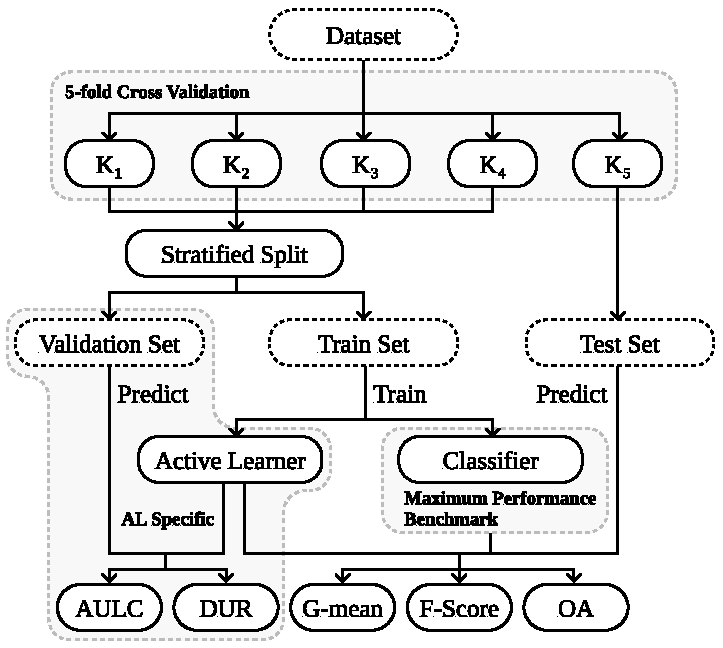
\includegraphics[width=.6\linewidth]{../analysis/experimental_procedure}
    \caption{%
        Experimental procedure flowchart.
    }~\label{fig:experimental_procedure}
\end{figure}

\subsection{Software Implementation}~\label{sec:software_implementation}

The experiment was implemented using the Python programming language, along
with the Python libraries
\href{https://scikit-learn.org/stable/}{Scikit-Learn}~\cite{Pedregosa2011},
\href{https://imbalanced-learn.org/en/stable/}{Imbalanced-Learn}~\cite{JMLR:v18:16-365},
\href{https://geometric-smote.readthedocs.io/en/latest/?badge=latest}{Geometric-SMOTE}~\cite{Douzas2019},
\href{https://research-learn.readthedocs.io/en/latest/?badge=latest}{Research-Learn}
and
\href{https://mlresearch.readthedocs.io/en/latest/?badge=latest}{ML-Research}
libraries. All functions, algorithms, experiments and results are provided in
the \href{https://github.com/joaopfonseca/ml-research/}{GitHub repository of
the project}.

\section{Results \& Discussion}~\label{sec:results_discussion}

\subsection{Results}~\label{sec:sub_results}


% TODO: Captions need to be rewritten

\begin{table}[H]
    \centering
    \pgfplotstabletypeset[
        col sep=comma,
        string type,
        every head row/.style={%
            before row=\toprule,
            after row=\midrule
        },
        every last row/.style={after row=\bottomrule},
    ]{../analysis/mean_std_aulc_ranks.csv}
    \caption{%
        Mean rankings of the AULC metric over the different datasets (7),
        folds (5) and runs (3) used in the experiment. This means that the use
        of G-SMOTE almost always improves the results of the original
        framework.
    }\label{tab:aulc_ranks}
\end{table}


\begin{table}[htb]
    \centering
    \pgfplotstabletypeset[
        col sep=comma,
        string type,
        every head row/.style={%
            before row=\toprule,
            after row=\midrule
        },
        every last row/.style={after row=\bottomrule},
    ]{../analysis/mean_std_aulc_scores.csv}
    \caption{\label{tab:aulc_scores}
        Average AULC of each AL configuration tested. Each AULC score is
        calculated using the G-mean scores of each iteration in the validation
        set. By the end of the iterative process, each AL configuration used a
        total of 750 instances of the 960 instances that compose the training
        set.
    }
\end{table}

\begin{table}[H]
    \centering
    \addtolength{\leftskip} {-2cm}
    \addtolength{\rightskip}{-2cm}
    \pgfplotstabletypeset[
        col sep=comma,
        string type,
        every head row/.style={%
            before row=\toprule,
            after row=\midrule
        },
        every last row/.style={after row=\bottomrule},
    ]{../analysis/optimal_data_utilization.csv}
    \caption{\label{tab:optimal_data_utilization}
        Mean data utilization of AL algorithms, as a percentage of the
        training set.
    }
\end{table}

\begin{figure}[H]
	\centering
	\includegraphics[width=1\linewidth]{../analysis/data_utilization_rate}
    \caption{%
        Mean data utilization rates. The y-axis shows the percentage of data
        (relative to the baseline AL framework) required to reach the
        different performance thresholds.
    }~\label{fig:dur}
\end{figure}


\begin{table}[H]
    \centering
    \addtolength{\leftskip} {-2cm}
    \addtolength{\rightskip}{-2cm}
    \pgfplotstabletypeset[
        col sep=comma,
        string type,
        every head row/.style={%
            before row=\toprule,
            after row=\midrule
        },
        every last row/.style={after row=\bottomrule},
    ]{../analysis/optimal_mean_std_scores.csv}
    \caption{\label{tab:optimal_mean_std_scores}
        Optimal classification scores. The Maximum Performance (MP)
        classification scores are calculated using classifiers trained using
        the entire training set.
    }
\end{table}


% \begin{table}[H]
%     \centering
%     \pgfplotstabletypeset[
%         col sep=comma,
%         string type,
%         every head row/.style={%
%             before row=\toprule,
%             after row=\midrule
%         },
%         every last row/.style={after row=\bottomrule},
%     ]{../analysis/wide_optimal_aulc.csv}
%     \caption{\label{tab:wide_optimal_aulc}
%         AULC scores of each AL configuration tested over the different
%         datasets. Each AULC score is calculated using the G-mean scores of
%         each iteration in the validation set. By the end of the iterative
%         process, each AL configuration used a total of 750 instances of the
%         960 instances that compose the training set.
%     }
% \end{table}


\subsection{Statistical Analysis}~\label{sec:statistical-analysis}


\begin{table}[htb]
	\centering
    \pgfplotstabletypeset[
        col sep=comma,
        string type,
        every head row/.style={%
            before row=\toprule,
            after row=\midrule
        },
        every last row/.style={after row=\bottomrule},
    ]{../analysis/wilcoxon_test.csv}
    \caption{%
    	Adjusted p-values using the Wilcoxon signed-rank method. Bold values
        are statistically significant at a level of $\alpha = 0.05$. The 
        null hypothesis is that the performance of the proposed
        framework is similar to that of the original framework.
    }\label{tab:wilcoxon_test}
\end{table}

% TODO: add analysis of dataset complexity versus AL performance


\subsection{Discussion}~\label{sec:sub_discussion}

\section{Conclusion}~\label{sec:conclusion}


\bibliography{references}
\bibliographystyle{ieeetr}

\end{document}
